% Created 2023-11-10 vie 20:50
% Intended LaTeX compiler: pdflatex
\documentclass[aspectratio=169, usenames,svgnames,dvipsnames]{beamer}
\usepackage[utf8]{inputenc}
\usepackage[T1]{fontenc}
\usepackage{graphicx}
\usepackage{longtable}
\usepackage{wrapfig}
\usepackage{rotating}
\usepackage[normalem]{ulem}
\usepackage{amsmath}
\usepackage{amssymb}
\usepackage{capt-of}
\usepackage{hyperref}
\usepackage{color}
\usepackage{listings}
\usepackage{mathpazo}
\usepackage{gensymb}
\usepackage{amsmath}
\usepackage{diffcoeff}
\usepackage{steinmetz}
\usepackage{mathtools}
\bibliographystyle{plain}
\usepackage{siunitx}
\sisetup{output-decimal-marker={,}}
\DeclareSIUnit{\watthour}{Wh}
\hypersetup{colorlinks=true, linkcolor=Blue, urlcolor=Blue}
\usepackage[symbol, perpage]{footmisc}
\newcommand{\laplace}[1]{\mathbf{#1}(\mathbf{s})}
\newcommand{\slp}{\mathbf{s}}
\newcommand{\fasor}[1]{\mathbf{#1}(\omega)}
\newcommand{\atan}{\mathrm{atan}}
\parskip=5pt
\usetheme{Boadilla}
\usecolortheme{rose}
\usefonttheme{serif}
\author{Oscar Perpiñán Lamigueiro}
\date{}
\title{Técnicas Generales de Análisis}
\subtitle{Teoría de Circuitos II}
\setbeamercolor{alerted text}{fg=blue!50!black} \setbeamerfont{alerted text}{series=\bfseries}
\AtBeginSubsection[]{\begin{frame}[plain]\tableofcontents[currentsubsection,sectionstyle=show/shaded,subsectionstyle=show/shaded/hide]\end{frame}}
\AtBeginSection[]{\begin{frame}[plain]\tableofcontents[currentsection,hideallsubsections]\end{frame}}
\beamertemplatenavigationsymbolsempty
\setbeamertemplate{footline}[frame number]
\setbeamertemplate{itemize items}[triangle]
\setbeamertemplate{enumerate items}[circle]
\setbeamertemplate{section in toc}[circle]
\setbeamertemplate{subsection in toc}[circle]
\hypersetup{
 pdfauthor={Oscar Perpiñán Lamigueiro},
 pdftitle={Técnicas Generales de Análisis},
 pdfkeywords={},
 pdfsubject={},
 pdfcreator={Emacs 29.1 (Org mode 9.6.11)}, 
 pdflang={Spanish}}
\begin{document}

\maketitle

\section{Leyes de Kirchhoff}
\label{sec:orge4607b7}

\begin{frame}[label={sec:org1c269a1}]{Nudo, rama, malla}
\begin{description}
\item[{Nudo}] unión de \alert{3} o más conductores.
\item[{Rama}] elementos conectados entre dos nudos consecutivos.
\item[{Lazo}] conjunto de ramas que forman un camino cerrado.
\item[{Malla}] lazo que no contiene ningún otro en su interior.
\end{description}

\begin{center}
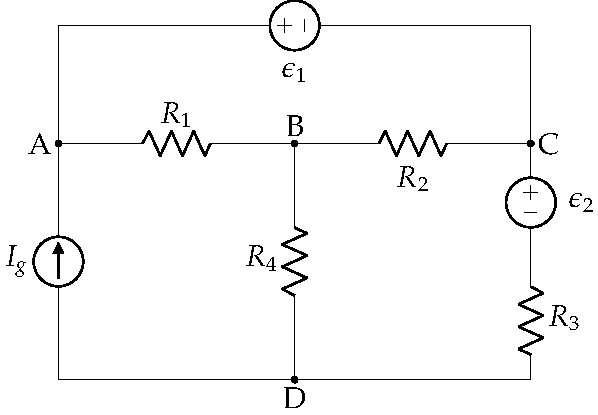
\includegraphics[height=0.5\textheight]{../figs/mallas.pdf}
\end{center}
\end{frame}

\begin{frame}[label={sec:orgb6e8447}]{Ley de Kirchhoff de las Corrientes (LKC)}
\begin{itemize}
\item La \alert{LKC} es el principio de conservación de la carga aplicado a los circuitos eléctricos.

\item \alert{LKC}: la suma de las corrientes que llegan a un nudo es igual a la suma de las que salen.

\begin{itemize}
\item Las lineas de corriente son cerradas (o solenoidales).
\end{itemize}
\end{itemize}

\begin{center}
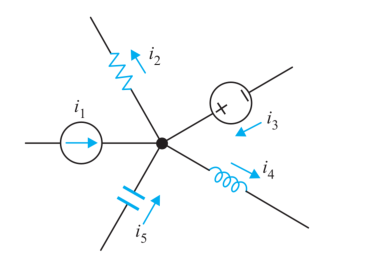
\includegraphics[height=0.4\textheight]{../figs/LKC_FM.pdf}
\end{center}
\[
i_1(t) - i_2(t) + i_3(t) - i_4(t) + i_5(t) = 0
\]
\end{frame}

\begin{frame}[label={sec:org6ff42a6}]{Ley de Kirchhoff de los Voltajes (LKV)}
\begin{itemize}
\item La \alert{LKV} es el principio de conservación de la energía aplicado a los circuitos eléctricos.

\item \alert{LKV}: la suma (con signo) de las tensiones a lo largo de un camino cerrado (circuito) es cero.

\begin{itemize}
\item La energía producida por un generador es consumida por los receptores del circuito para producir trabajo (mecánico, químico, etc.) o calor.
\end{itemize}
\end{itemize}

\begin{center}
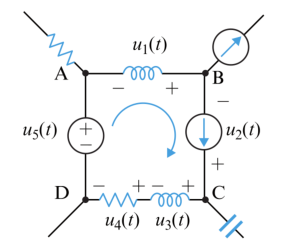
\includegraphics[height=0.4\textheight]{../figs/LKV_FM.pdf}
\end{center}
\[
u_3(t) + u_4 (t) - u_5 (t) - u_1 (t) - u_2 (t)  = 0
\]
\end{frame}

\subsection{Asociación de condensadores}
\label{sec:org5a7cd6d}

\begin{frame}[label={sec:org07c80be}]{Zona aislada}
En una asociación de condensadores aparecen zonas aisladas (puntos a los que no se puede llegar sin atravesar un condensador.)

\begin{center}
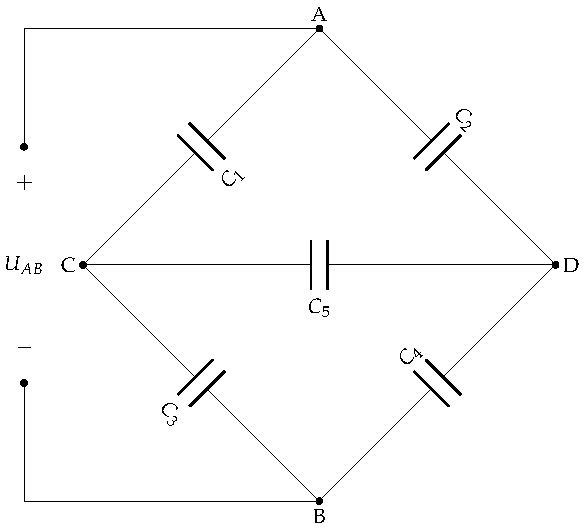
\includegraphics[height=0.6\textheight]{../figs/CondensadoresZonaAislada.pdf}
\end{center}
\end{frame}

\begin{frame}[label={sec:orga305442}]{Zona aislada}
\begin{itemize}
\item La tensión en estas zonas aisladas \alert{no se puede determinar de forma directa} a partir del resto del circuito.
\item Cuando la carga inicial de todos los condensadores es nula \alert{y} la asociación se puede sustituir por un condensador equivalente \(C_{eq}\) (serie, paralelo):
\begin{itemize}
\item La carga de \(C_{eq}\) se calcula a partir de la tensión de la asociación.
\item \alert{Asociaciones serie}:
\begin{itemize}
\item La carga de los condensadores individuales es igual a la de  \(C_{eq}\).
\item La tensión de \(C_{eq}\) es la suma de las tensiones individuales.
\end{itemize}
\item \alert{Asociaciones paralelo}:
\begin{itemize}
\item La carga de \(C_{eq}\) se reparte entre los condensadores individuales.
\item La tensión de \(C_{eq}\) es igual a la de los condensadores individuales.
\end{itemize}
\end{itemize}
\item El resto de casos se resuelven combinando ecuaciones de nudos y mallas.
\end{itemize}
\end{frame}

\begin{frame}[label={sec:orgf50f618}]{Método de resolución (1)}
Se asignan polaridades arbitrarias a los condensadores.

\begin{center}
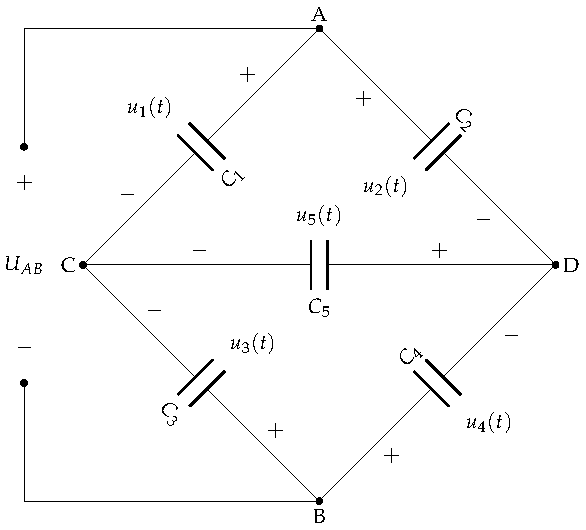
\includegraphics[height=0.8\textheight]{../figs/CondensadoresZonaAislada_Tensiones.pdf}
\end{center}
\end{frame}

\begin{frame}[label={sec:org5171c8e}]{Método de resolución (2)}
La suma de cargas en una zona aislada es igual a la suma total de las cargas iniciales (nula si los condensadores no tienen carga inicial).
\begin{columns}
\begin{column}{0.5\columnwidth}
\begin{center}
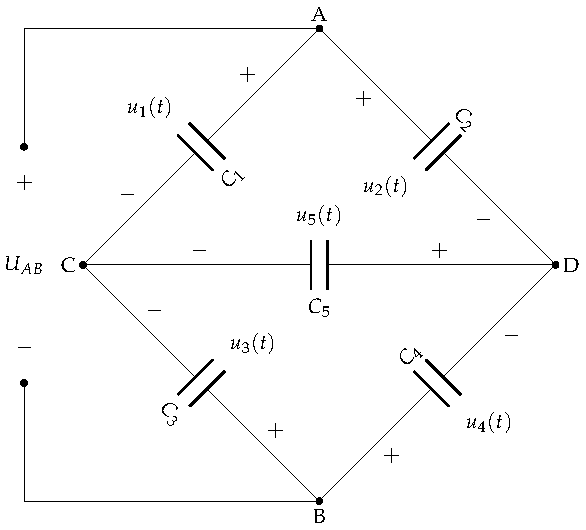
\includegraphics[height=0.75\textheight]{../figs/CondensadoresZonaAislada_Tensiones.pdf}
\end{center}
\end{column}
\begin{column}{0.5\columnwidth}
\begin{align*}
  (C) &\quad q_1 + q_5 + q_3 = 0\\
  (D) &\quad q_5 - q_2 - q_4 = 0
\end{align*}
\end{column}
\end{columns}
\end{frame}

\begin{frame}[label={sec:orgc700916}]{Método de resolución (3)}
Se aplica la LKV a las mallas que sean necesarias para completar el sistema de ecuaciones (usando \(u_{Ci} = q_i/C_i\)).
\begin{columns}
\begin{column}{0.5\columnwidth}
\begin{center}
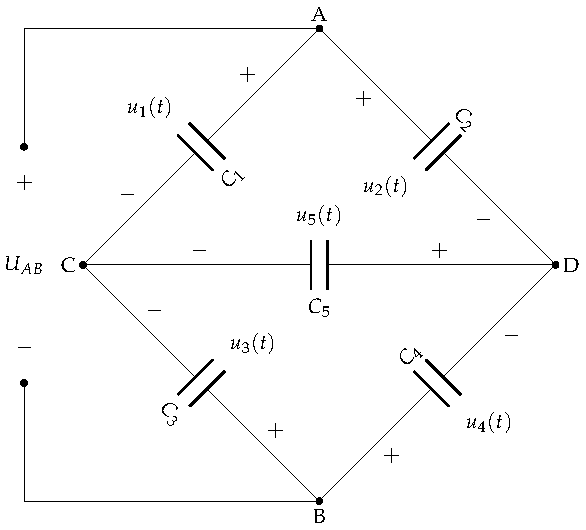
\includegraphics[height=0.75\textheight]{../figs/CondensadoresZonaAislada_Tensiones.pdf}
\end{center}
\end{column}
\begin{column}{0.5\columnwidth}
\begin{align*}
  (ACDA) &\quad \frac{q_1}{C_1} - \frac{q_5}{C_5} - \frac{q_2}{C_2} = 0\\
  (CBDC) &\quad -\frac{q_3}{C_3} + \frac{q_4}{C_4} + \frac{q_5}{C_5} = 0\\
  (ACBA) &\quad \frac{q_1}{C_1} - \frac{q_3}{C_3} - u_{AB} = 0
\end{align*}
\end{column}
\end{columns}
\end{frame}

\begin{frame}[label={sec:orge6fbda3}]{Método de resolución (y 4)}
Se resuelve el sistema de ecuaciones para obtener los valores de \(q_i\).

\begin{align*}
  q_1 + q_5 + q_3 &= 0\\
  q_5 - q_2 - q_4 &= 0\\
  \frac{q_1}{C_1} - \frac{q_5}{C_5} - \frac{q_2}{C_2} &= 0\\
  -\frac{q_3}{C_3} + \frac{q_4}{C_4} + \frac{q_5}{C_5} &= 0\\
  \frac{q_1}{C_1} - \frac{q_3}{C_3} &= u_{AB}
\end{align*}
\end{frame}



\section{Métodos de Análisis}
\label{sec:org9df1b0b}

\subsection{Método de las mallas}
\label{sec:org143fe50}

\begin{frame}[label={sec:org869ba04}]{}
\begin{center}
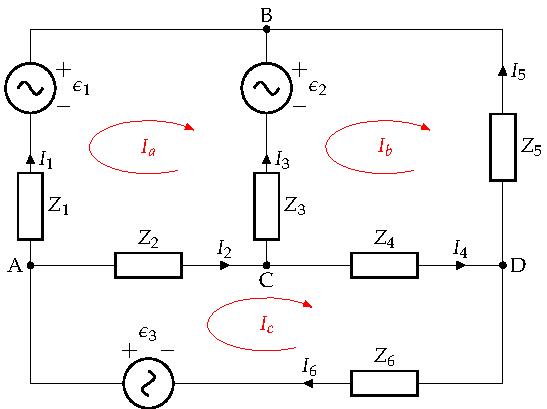
\includegraphics[height=0.95\textheight]{../figs/mallas_alterna.pdf}
\end{center}
\end{frame}

\begin{frame}[label={sec:org5347b38}]{Ecuación General}
\begin{equation*}
  \begin{bmatrix}
    {\color{BrickRed}\sum \overline{Z}_{aa}} &  - {\color{MidnightBlue}\sum \overline{Z}_{ab}} & - {\color{MidnightBlue}\sum \overline{Z}_{ca}} \\
    - {\color{MidnightBlue}\sum \overline{Z}_{ab}} & {\color{BrickRed}\sum \overline{Z}_{bb}} & - {\color{MidnightBlue}\sum \overline{Z}_{bc}} \\
    - {\color{MidnightBlue}\sum \overline{Z}_{ca}} & - {\color{MidnightBlue}\sum \overline{Z}_{bc}} &  {\color{BrickRed}\sum \overline{Z}_{cc}}
  \end{bmatrix} \cdot %
  \begin{bmatrix}
    \overline{I}_a\\
    \overline{I}_b\\
    \overline{I}_c\\
  \end{bmatrix} = %
  \begin{bmatrix}
    {\color{OliveGreen}\sum\overline{\epsilon}_a}\\
    {\color{OliveGreen}\sum\overline{\epsilon}_b}\\
    {\color{OliveGreen}\sum\overline{\epsilon}_c}
  \end{bmatrix}
\end{equation*}
\begin{description}
\item[{\({\color{BrickRed}\sum \overline{Z}_{aa}}\)}] suma de las impedancias incluidas en la malla de \(\overline{I}_a\).
\item[{\({\color{MidnightBlue}\sum \overline{Z}_{ab}}\)}] suma de las impedancias incluidas en las ramas compartidas por las mallas de \(\overline{I}_a\) e \(\overline{I}_b\).
\item[{\({\color{OliveGreen}\sum \overline{\epsilon}_a}\)}] suma algebraica de las fuerzas electromotrices de los generadores de la malla de \(\overline{I}_a\). Su signo es positivo si contribuyen al giro de la corriente.
\end{description}
\end{frame}
\begin{frame}[label={sec:org9f69c2f}]{Procedimiento}
\begin{enumerate}
\item Identificar las corrientes de rama.
\item Asignar un sentido a las corrientes de malla.
\item Relacionar corrientes de rama con corrientes de malla.
\item Escribir ecuación de mallas.
\item Resolver la ecuación, obteniendo las corrientes de malla.
\item Obtener las corrientes de rama con las relaciones del punto 3.
\end{enumerate}

\alert{Importante}: todos los generadores deben ser fuentes de tensión.
\end{frame}

\begin{frame}[label={sec:orgea51b16}]{Admitancia generalizada}
\begin{equation*}
  \begin{bmatrix}
    \overline{Z}_{11} & \overline{Z}_{12} & \dots & \overline{Z}_{1n} \\
    \overline{Z}_{21} & \overline{Z}_{22} & \dots & \overline{Z}_{2n} \\
    \vdots & \vdots & \ddots & \vdots \\
    \overline{Z}_{n1} & \overline{Z}_{n2} &  \dots & \overline{Z}_{nn}
  \end{bmatrix} \cdot %
  \begin{bmatrix}
    \overline{I}_1\\
    \overline{I}_2\\
    \vdots \\
    \overline{I}_n\\
  \end{bmatrix} = %
  \begin{bmatrix}
    \overline{\epsilon}_1\\
    \overline{\epsilon}_2\\
    \vdots \\
    \overline{\epsilon}_n
  \end{bmatrix}
\end{equation*}
Aplicando la regla de Cramer
\[
  \overline{I}_k = \overline{\epsilon}_1 \frac{\Delta_{1k}}{|Z|} + \overline{\epsilon}_2 \frac{\Delta_{2k}}{|Z|} + \dots + \overline{\epsilon}_n \frac{\Delta_{nk}}{|Z|}
\]
siendo \(\Delta_{ij}\) el adjunto del elemento \(ij\) de la matriz \(Z\):
\[
  \Delta_{ij} = (-1)^{i+j} \cdot |M_{ij}|
\]
donde \(M_{ij}\) es la matriz resultante de eliminar la fila \(i\) y la columna \(j\) de la matriz \(Z\).
\end{frame}

\begin{frame}[label={sec:orgc454be2}]{Admitancia generalizada}
Esta expresión indica que las respuestas del circuito (\(I_k\)) dependen de todas las excitaciones que existan (\(\epsilon_i\)):
\[
  \overline{I}_k = \overline{\epsilon}_1 \frac{\Delta_{1k}}{|Z|} + \overline{\epsilon}_2 \frac{\Delta_{2k}}{|Z|} + \dots + \overline{\epsilon}_n \frac{\Delta_{nk}}{|Z|}
\]
También se puede definir la admitancia generalizada entre dos partes del circuito:
\[
  \overline{Y}_{ik} = \frac{\overline{I}_k}{\overline{\epsilon}_i} = \frac{\Delta_{ik}}{|Z|}
\]
\end{frame}

\begin{frame}[label={sec:org9faa8a0}]{Impedancia de Entrada}
A partir de esta expresión se puede calcular la impedancia de entrada vista por una fuente que alimenta un circuito pasivo (todas las fuentes salvo la de entrada son nulas en la expresión anterior):

\[
  \overline{I}_1 = \overline{\epsilon}_1 \frac{\Delta_{11}}{|Z|} + 0 \cdot \frac{\Delta_{21}}{|Z|} + \dots + 0 \cdot \frac{\Delta_{n1}}{|Z|}
\]
Por tanto:
\[
  \boxed{\overline{Z}_{in} = \frac{\overline{\epsilon}_1}{\overline{I}_1}=  \frac{|Z|}{\Delta_{11}}}
\]
\end{frame}

\begin{frame}[label={sec:org999af05}]{Impedancia de Transferencia}
También se puede calcular la impedancia de transferencia de un circuito pasivo, es decir, la impedancia entre dos partes del circuito en las que la primera está alimentada por una fuente, y la segunda está cortocircuitada.

En este caso, todas las fuentes salvo la de interés están apagadas:

\[
  \overline{I}_k = 0 \cdot \frac{\Delta_{1k}}{|Z|} + 0 \cdot \frac{\Delta_{2k}}{|Z|} + \dots + \epsilon_j \cdot \frac{\Delta_{jk}}{|Z|} + 0 \cdot \frac{\Delta_{nk}}{|Z|}
\]
Por tanto:
\[
  \boxed{\overline{Z}_{Tjk} = \frac{\overline{\epsilon}_j}{\overline{I}_k}=  \frac{|Z|}{\Delta_{jk}}}
\]
\end{frame}


\begin{frame}[label={sec:orga6a3844}]{Mallas con fuentes dependientes}
\begin{itemize}
\item Se plantean las ecuaciones de mallas como si no hubiese fuentes dependientes.
\item Se añade la ecuación de la fuente dependiente como una ecuación adicional.
\item La matriz de impedancias \alert{deja de ser simétrica}.
\end{itemize}
\end{frame}

\begin{frame}[label={sec:orgaa29f4f}]{Mallas con fuentes de intensidad ideales}
\begin{itemize}
\item Si la fuente de corriente está en una \alert{rama que pertenece a una única malla}, se fija la corriente de dicha malla igual a la corriente de la fuente (desaparece una incógnita del sistema).
\item Si la fuente de corriente está en una \alert{rama que pertenece a dos mallas}:
\begin{itemize}
\item Se introduce la tensión en la fuente de corriente como variable adicional.
\item Se plantean las ecuaciones del método de mallas.
\item La variable adicional (tensión de la fuente) se elimina sumando las dos ecuaciones de las mallas afectadas.
\item Se añade una ecuación que relaciona la corriente de la fuente con las dos corrientes de malla.
\end{itemize}
\end{itemize}
\end{frame}

\subsection{Método de los nudos}
\label{sec:orgb31e3c6}
\begin{frame}[label={sec:org75fb807}]{}
\begin{center}
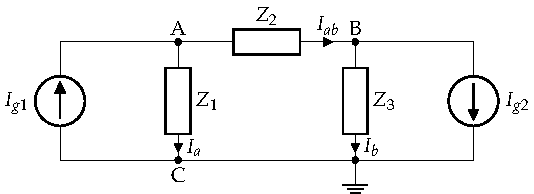
\includegraphics[width=.9\linewidth]{../figs/nudosAC.pdf}
\end{center}
\end{frame}

\begin{frame}[label={sec:org9073cac}]{Ecuación general}
\begin{equation*}
  \begin{bmatrix}
    {\color{BrickRed}\sum \overline{Y}_A} & - {\color{MidnightBlue}\sum \overline{Y}_{AB}} & - {\color{MidnightBlue}\sum \overline{Y}_{AC}}\\
    -{\color{MidnightBlue}\sum \overline{Y}_{AB}} & {\color{BrickRed}\sum \overline{Y}_B} & -{\color{MidnightBlue}\sum \overline{Y}_{BC}}\\
    -{\color{MidnightBlue}\sum \overline{Y}_{AC}} & -{\color{MidnightBlue}\sum \overline{Y}_{BC}} & {\color{BrickRed}\sum \overline{Y}_C}
  \end{bmatrix} \cdot%
  \begin{bmatrix}
    \overline{V}_A\\
    \overline{V}_B\\
    \overline{V}_C
  \end{bmatrix} = %
  \begin{bmatrix}
    {\color{OliveGreen}\sum \overline{I}_{gA}}\\
    {\color{OliveGreen}\sum \overline{I}_{gB}}\\
    {\color{OliveGreen}\sum \overline{I}_{gC}}
  \end{bmatrix}
\end{equation*}

\begin{description}
\item[{\({\color{BrickRed}\sum \overline{Y}_A}\)}] Suma de las admitancias conectadas al nudo \(A\).
\item[{\({\color{MidnightBlue}\sum \overline{Y}_{AB}}\)}] Suma de las admitancias conectadas entre los nudos \(A\) y \(B\).
\item[{\({\color{OliveGreen}\sum \overline{I}_{gA}}\)}] Suma de las corrientes de los generadores conectados en el nudo A. El signo es positivo si el generador inyecta corriente en el nudo.
\end{description}

\alert{Importante}: todos los generadores deben ser fuentes de corriente.
\end{frame}

\begin{frame}[label={sec:orgd91e2a4}]{Impedancia generalizada}
\begin{equation*}
  \begin{bmatrix}
    \overline{Y}_{11} & \overline{Y}_{12} & \dots & \overline{Y}_{1n} \\
    \overline{Y}_{21} & \overline{Y}_{22} & \dots & \overline{Y}_{2n} \\
    \vdots & \vdots & \ddots & \vdots \\
    \overline{Y}_{n1} & \overline{Y}_{n2} &  \dots & \overline{Y}_{nn}
  \end{bmatrix} \cdot %
  \begin{bmatrix}
    \overline{V}_1\\
    \overline{V}_2\\
    \vdots \\
    \overline{V}_n\\
  \end{bmatrix} = %
  \begin{bmatrix}
    \overline{I}_{g1}\\
    \overline{I}_{g2}\\
    \vdots \\
    \overline{I}_{gn}
  \end{bmatrix}
\end{equation*}
Aplicando la regla de Cramer
\[
  \overline{V}_k = \overline{I}_{g1} \frac{\Delta_{1k}}{|Y|} + \overline{I}_{g2} \frac{\Delta_{2k}}{|Y|} + \dots + \overline{I}_{gn} \frac{\Delta_{nk}}{|Y|}
\]
siendo \(\Delta_{ij}\) el adjunto del elemento \(ij\) de la matriz \(Y\):
\[
  \Delta_{ij} = (-1)^{i+j} \cdot |M_{ij}|
\]
donde \(M_{ij}\) es la matriz resultante de eliminar la fila \(i\) y la columna \(j\) de la matriz \(Y\).
\end{frame}

\begin{frame}[label={sec:org8bf3b8d}]{Impedancia generalizada}
Esta expresión indica que las respuestas del circuito (\(V_k\)) dependen de todas las excitaciones que existan (\(I_{gi}\)):
\[
  \overline{V}_k = \overline{I}_{g1} \frac{\Delta_{1k}}{|Y|} + \overline{I}_{g2} \frac{\Delta_{2k}}{|Y|} + \dots + \overline{I}_{gn} \frac{\Delta_{nk}}{|Y|}
\]
También se puede definir la impedancia generalizada entre dos partes del circuito:
\[
  \overline{Z}_{ik} = \frac{\overline{V}_k}{\overline{I}_{gi}} = \frac{\Delta_{ik}}{|Y|}
\]
\end{frame}

\begin{frame}[label={sec:org4c4f6f1}]{Admitancia de Entrada}
A partir de esta expresión se puede calcular la admitancia de entrada vista por una fuente que alimenta un circuito pasivo (todas las fuentes salvo la de entrada son nulas en la expresión anterior):

\[
  \overline{V}_1 = \overline{I}_{g1} \frac{\Delta_{11}}{|Y|} + 0 \cdot \frac{\Delta_{21}}{|Y|} + \dots + 0 \cdot \frac{\Delta_{n1}}{|Y|}
\]
Por tanto:
\[
  \boxed{\overline{Y}_{in} = \frac{\overline{I}_{g1}}{\overline{V}_1}=  \frac{|Y|}{\Delta_{11}}}
\]
\end{frame}

\begin{frame}[label={sec:orga3da0f2}]{Admitancia de Transferencia}
También se puede calcular la admitancia de transferencia de un circuito pasivo, es decir, la admitancia entre dos partes del circuito en las que la primera está alimentada por una fuente, y la segunda está en abierto.

En este caso, todas las fuentes salvo la de interés están apagadas:

\[
  \overline{V}_k = 0 \cdot \frac{\Delta_{1k}}{|Y|} + 0 \cdot \frac{\Delta_{2k}}{|Y|} + \dots + I_{gj} \cdot \frac{\Delta_{jk}}{|Y|} + 0 \cdot \frac{\Delta_{nk}}{|Y|}
\]
Por tanto:
\[
  \boxed{\overline{Y}_{Tjk} = \frac{\overline{I}_{gj}}{\overline{V}_k}=  \frac{|Y|}{\Delta_{jk}}}
\]
\end{frame}


\begin{frame}[label={sec:org4820703}]{Nudos con fuentes dependientes}
\begin{itemize}
\item Se plantean las ecuaciones de nudos como si no hubiese fuentes dependientes.
\item Se añade la ecuación de la fuente dependiente como una ecuación adicional.
\item La matriz de admitancias deja de ser simétrica.
\end{itemize}
\end{frame}


\begin{frame}[label={sec:orgf1bbc92}]{Nudos con fuentes de tensión ideales}
\begin{itemize}
\item Si la fuente de tensión está \alert{conectada entre el nudo de referencia y otro nudo cualquiera}, se fija la tensión de este último igual a la tensión de la fuente.
\item Si la fuente de tensión está \alert{conectada entre dos nudos}, no siendo ninguno de ellos de referencia:
\begin{itemize}
\item Se introduce la corriente que atraviesa la fuente como variable adicional.
\item Se plantean las ecuaciones del método de nudos.
\item Se elimina la variable adicional (corriente de la fuente de tensión) sumando las ecuaciones de nudos afectadas.
\item Se añade una ecuación que relaciona la tensión de la fuente con las dos tensiones nodales.
\end{itemize}
\end{itemize}
\end{frame}

\begin{frame}[label={sec:org91a649f}]{Nudos con fuentes de tensión ideales: supernudos}
Si la fuente de tensión está conectada entre dos nudos, no siendo ninguno de ellos de referencia, estos dos nudos se pueden considerar como un único \alert{supernudo}:
\begin{itemize}
\item Este supernudo no tiene tensión propia.
\item Se plantean las ecuaciones de nudos incluyendo el supernudo (pero diferenciando los nudos implicados en el supernudo).
\item El supernudo aporta una ecuación adicional, la tensión de la fuente que contiene.
\end{itemize}
\end{frame}


\begin{frame}[label={sec:org3eed2fc}]{Ejemplo de supernudo}
\begin{center}
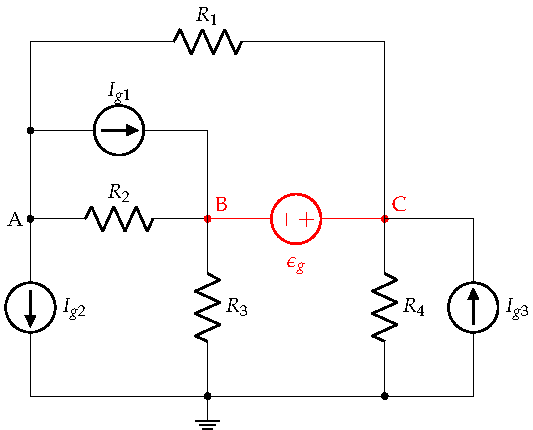
\includegraphics[height=0.5\textheight]{../figs/supernudo.pdf}
\end{center}

\begin{align*}
  V_a\cdot (\frac{1}{R_1} + \frac{1}{R_2}) - V_b \cdot \frac{1}{R_2} - V_c \cdot \frac{1}{R_1} &= -I_{g1} - I_{g2} \quad (A)\\
  - V_a\cdot (\frac{1}{R_1} + \frac{1}{R_2}) + V_b \cdot (\frac{1}{R_2} + \frac{1}{R_3}) + V_c \cdot (\frac{1}{R_1} + \frac{1}{R_4}) &= I_{g1} + I_{g3} \quad (BC)\\
  V_c - V_b &= \epsilon_g
\end{align*}
\end{frame}
\end{document}
